% !TEX root = _main.tex

% ==========================================
% ここから本文．あとは各自で
% ==========================================

%1
\section{はじめに}

近年インターネットの普及に伴い音楽の楽しみ方が大きく変化している．
従来ではCDを購入してプレイヤーで楽しむことが一般的であったが，近年はインターネット配信で楽しむ人が増加している．
各音楽配信サイトなどでは，ユーザの嗜好に合った楽曲の検索を容易にするために楽曲を音楽ジャンル別で分類されることが多くみられる．

しかし，楽曲のジャンルは時系列で変わっていくのではないだろうか？

例として，「Mrs. GREEN APPLE」の「ライラック」\cite{lilac}があげられる．
この楽曲は，冒頭約10秒間でギターにエフェクトを加えた電子音が流れる．
しかし，その後同じフレーズをドラムやギターの音色で構成する．
これにより，電子音のような音色では感じることのなかったロックミュージックの印象を抱かせるものとなっている．
このように，聴取する箇所によって抱く印象が異なる楽曲が存在すると考える．

また，音楽ジャンル解析は古くから数多くの研究が行われており，近年では主要な研究テーマの１つとして扱われている．
しかし，これらの大半は１つの楽曲を1つの音楽ジャンルに分類するものである．
このような音楽ジャンルの分類方法では，楽曲内における音楽ジャンルの変化の識別が困難であると考える．

そこで本研究では，数ある音響特徴量の中でも音色に着目し，対象楽曲の楽器構成から音楽ジャンルの変化を時系列で表示するシステムを提案することを目的とする．




%2
\section{先行研究}
現在まで，音楽ジャンル解析に関する研究は数多く行われている．楽曲のパート編成やピッチ，音長，リズムパターン，音色，リズム特性などといった特徴量を対象とした研究がある．

土橋らは音響信号の中でもベースパートに着目し，ベースパートの特徴量，音色，リズムを用いた音楽ジャンル推定を行っている\cite{bassline}．また，鈴木らは旋律パートのみを用いて音楽ジャンル判別を行うための新たな特徴量を提案し，その有効性を検証している\cite{melody}．

Basiliら\cite{basili}はMIDIデータから楽曲のパート編成やピッチ，音長といった高次の特徴量を抽出し，機械学習アルゴリズムを用いて音楽ジャンルを分類している．

上記で記した研究は１つの楽曲に対して１つのジャンルを判別するものであり，従来はこの判別方法が典型であった．しかし，本研究では楽曲を時間で区切ることにより，楽曲内の音楽ジャンルの変化を可視化することが可能となる．



\section{研究概要}
\figref{fig:system}は，提案システムのシステム構成図である．

\begin{figure}[tb]
	  \centering
	  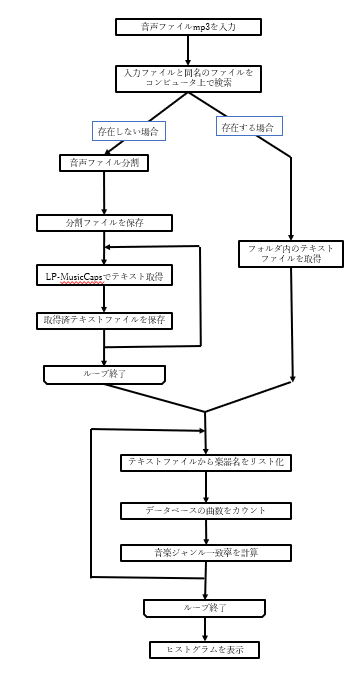
\includegraphics[width=\hsize]{fig/fig18-sistem.png}
	  \caption{システム構成図}
	  \label{fig:system}
\end{figure}

分析する楽曲を対象楽曲とし，対象楽曲の入力ファイルは.mp3形式を想定する．
分析結果はジャンルごとにヒストグラムで表示する．

提案システムの構成は主に音色の抽出，音楽ジャンルの解析，計算結果の表示の３つにわけることが出来る．
データベースと入力データの前処理について記述した後，システムの詳細を記述する．

\subsection{データベース}
音楽ジャンル分析には，独自に収集したデータセットを使用する．
jazz，classic，rockの３ジャンルを対象とし，各ジャンル50曲，合計150曲の楽曲を選定した．
使用楽曲は，音楽配信サービスSpotifyにて各ジャンルの名盤を検索し，人気順で選定した．
また，正確なジャンル分類を保証するため，Apple MusicおよびAmazon Musicといった他の音楽配信サービスのジャンル情報とも一致する楽曲のみを選定した．

楽曲情報はSpotifyを主なデータソースとし，スコアや楽曲クレジット情報を元に使用されている楽器構成を抽出した．
また，一部の楽曲についてスコアや詳細な楽曲クレジット情報が不足している場合には，聴取による推定や補足を行った．

なお，ソフトウェア音源やMIDI音源を使用して楽器の音色を再現している楽曲については，再現している楽器として抽出した．
また，楽器の音ではないシンセサイザについては，電子音とした．

作成したデータベースの一部を\figref{fig:database}に示す．

\begin{figure}[tb]
	  \centering
	  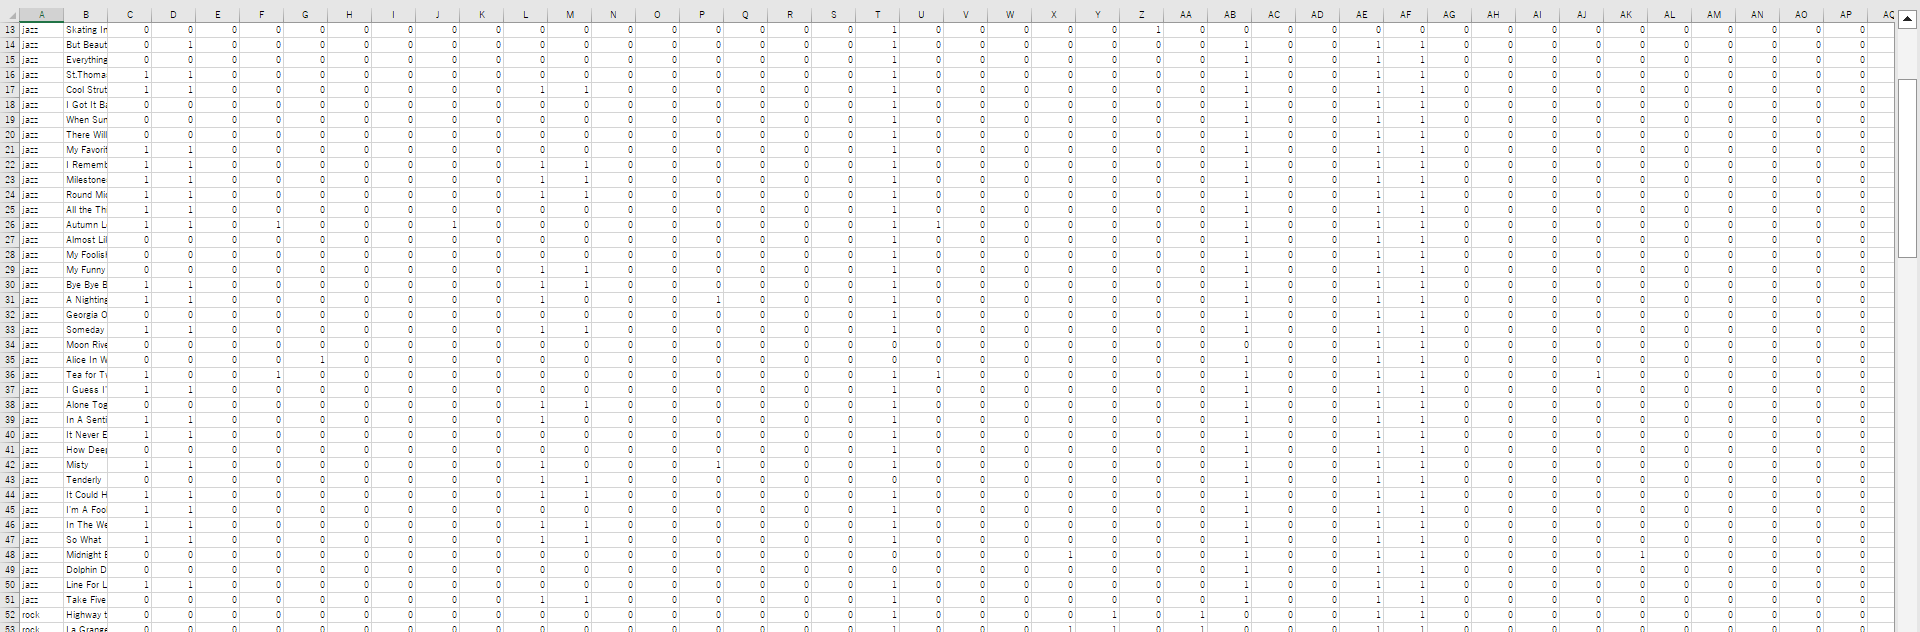
\includegraphics[width=\hsize]{fig/fig11-database.png}
	  \caption{データベース（一部）}
	  \label{fig:text}
\end{figure}

\subsection{データの前処理}
入力された音声ファイルを5秒ごとのセグメントに分割する．
音声ファイル名のフォルダを新たに作成し，作成フォルダ内に各セグメントを格納する．
音声ファイル名のフォルダが既に存在する場合には，この処理は行わずに既存のセグメントを解析に用いる．
これにより，データの重複を防ぐことが可能である．

\subsection{音色の抽出}
１はじめにで記述したように，本研究では時間水位における楽器構成の変化を捉え，対象楽曲の楽器構成から音楽ジャンルの変化を分析する．

音色の抽出にはLP-MusicCaps: LLM-Based Pseudo Music Captioning\cite{LP}を使用する．
これはISMIR 2023\cite{ISMIR2023}で発表されたもので，音楽トラックに対して自然言語によるキャプションを自動生成するものである．

表２は，LP-MusicCapsの整合性を示したものである．
使用楽器数が少ない楽曲では高い整合性があることがわかる．
しかし，楽器構成が複雑になるほど正確に抽出することが困難である傾向があると考える．

図２は音色の抽出手法のシステム構成図である．

LP-MusicCapsは音声データからテキスト生成するテキストである．
音声ファイルをLP-MusicCapsの外部webサイトを介して生成されたテキストを取得する．
LP-MusicCapsで生成されたテキストはセグメントが保存されているフォルダ内にテキストファイルとして保存される．

しかし，外部webサイトを介した処理を行う場合に処理速度が遅くなるという問題がある．
解決方法として，すでに入力音声ファイルと同名のフォルダが存在する場合にはLP-MusicCapsを介した処理を行わず，フォルダ内に存在するテキストファイルからテキストを取得する処理を追加した．
これにより，過去に解析したことのある楽曲を再度解析する際の処理速度が短縮される．

取得されたテキストから正規表現を用いて楽器名のみを抽出する処理を施し，解析したセグメントの楽器構成をリスト化して取得する．

以上の処理を各セグメントに対して行い，時間ごとの楽器構成を抽出する．

\subsection{音楽ジャンルの解析}
本研究では，対象楽曲の楽器構成と一致する楽器構成の楽曲がデータベースに何曲存在するかを計算した数値をジャンルの一致率と定義する．

一致率はジャンルごとに計算する．
ジャンルの一致率(G)の計算式は以下のとおりである．


ジャンルの一致率Gは最大値を１として，数値が大きいほど一致度が高いことを示す．

対象楽曲の楽器構成を取得すると，まずデータベースの各ジャンルの総楽曲数をカウントする．
次にデータベース上の楽曲から取得された楽器構成とマッチする楽曲をカウントし，上記の計算式を用いてジャンルの一致率を算出する．

上記の処理をセグメントごとに各ジャンル行う．

\subsection{計算結果の表示}
計算結果はヒストグラムで表示する．
一致率をジャンルごとのヒストグラムで可視化し，横軸をセグメント，縦軸を一致率とする．

また，TKinterを使用して，ユーザが音声ファイルの入力を安易に行えるようなGUIを作成した(\figref{GUI_start}，\figref{GUI_end})．

\begin{figure}[tb]
    \centering
    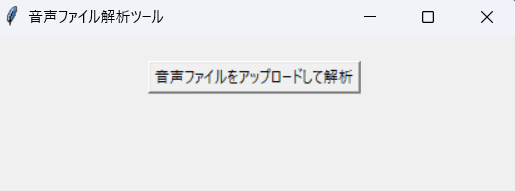
\includegraphics[width=\hsize]{fig/fig4-GUI_start.png}
    \caption{音声ファイル入力の画面}
    \label{GUI_start}
\end{figure}

\begin{figure}[tb]
    \centering
    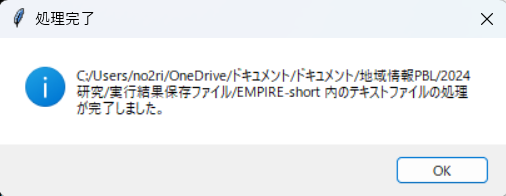
\includegraphics[width=\hsize]{fig/fig5-GUI_end.png}
    \caption{解析完了時の画面}
    \label{GUI_end}
\end{figure}



\section{実装の詳細}
本章では，作成したシステムの試用ライブラリと主要な関数についての解説を記述する．

\subsection{使用ライブラリ}
・os：ファイルやディレクトリの操作に使用するライブラリである．特に，フォルダ内のファイルリスト取得やパス操作に使用した．

・tkinter：GUIを構築するためのライブラリである．本システムでは，ファイルのアップロードや結果の表示に利用した．

・pandas：データフレーム形式でのデータ操作を効率化するライブラリである．本研究ではcsvファイルの読み込みやデータ集計の処理に利用した．

・re：正規表現を用いた文字列操作のライブラリである．本システムでは楽器名の抽出の際に利用した．

・matplotlib：データの可視化に関するライブラリである．本システムでは，結果をヒストグラムとして表示するために使用した．

\subsection{Calculate-genre-match-rate関数}
本関数は，楽器名リストとデータフレームを入力として受け取り，音楽ジャンルごとの一致率を計算する関数である．
関数のソースコードを\figref{fig:genre.match.rate}に示す．

\begin{figure}[tb]
	  \centering
	  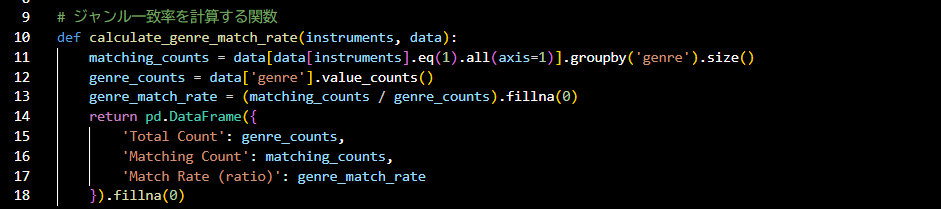
\includegraphics[width=\hsize]{fig/fig6-genre.match.rate.png}
	  \caption{Calculate-genre-match-rate関数のソースコード}
	  \label{fig:text}
\end{figure}

主な処理内容は以下のとおりである．

引数は”instruments”（楽器名リスト），”data”（データベース）である．

楽器列が１である行を抽出，フィルタリングし，音楽ジャンルごとに一致行をカウントする．
次に”genre”列全体の音楽ジャンルごとの総数をカウントし，カウントした総数と一致行数を用いて一致率を算出する．
計算式は３章で示した通りである．

出力は，以下の3つのカラムを持つデータフレームを返す．

・Total Count：ジャンルの総曲数

・Matching Count：楽器構成が一致している曲数

・Match Rate(ratio)：音楽ジャンルの一致率

\subsection{Plot-genre-histograms関数}
本関数は，音楽ジャンルごとのセグメントごとの一致率をヒストグラムで表示する関数である．

関数のソースコードを\figref{fig:genre.match.rate}に示す．

\begin{figure}[tb]
	  \centering
	  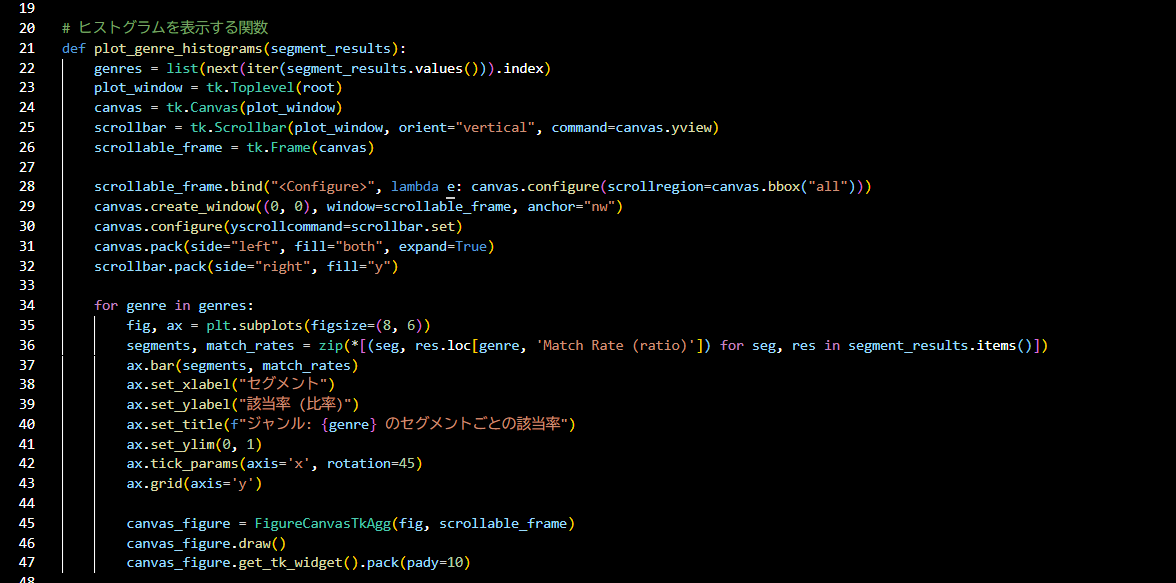
\includegraphics[width=\hsize]{fig/fig7-histgram.png}
	  \caption{Plot-genre-histograms関数のソースコード}
	  \label{fig:text}
\end{figure}

ヒストグラムの表示はtkinterライブラリを使用してサブウィンドウを表示して行う．引数は”segment-results”（各セグメントの音楽ジャンル該当率）である．

各セグメントにおける一致率を取得後，縦軸を音楽ジャンル一致率の最大値，横軸をセグメント（時間経過）としたヒストグラムをサブウィンドウに表示する．
サブウィンドウにはグラフ表示領域と垂直スクロールバーを作成し，フレーム内の要素が変化したときキャンバスのスクロール領域を自動調整する処理を追加している．

\subsection{Process-existing-folder関数}
本関数は，フォルダ内のテキストファイルを処理し，楽器名を抽出する関数である．

関数のソースコードを\figref{fig:folder}に示す．

\begin{figure}[tb]
	  \centering
	  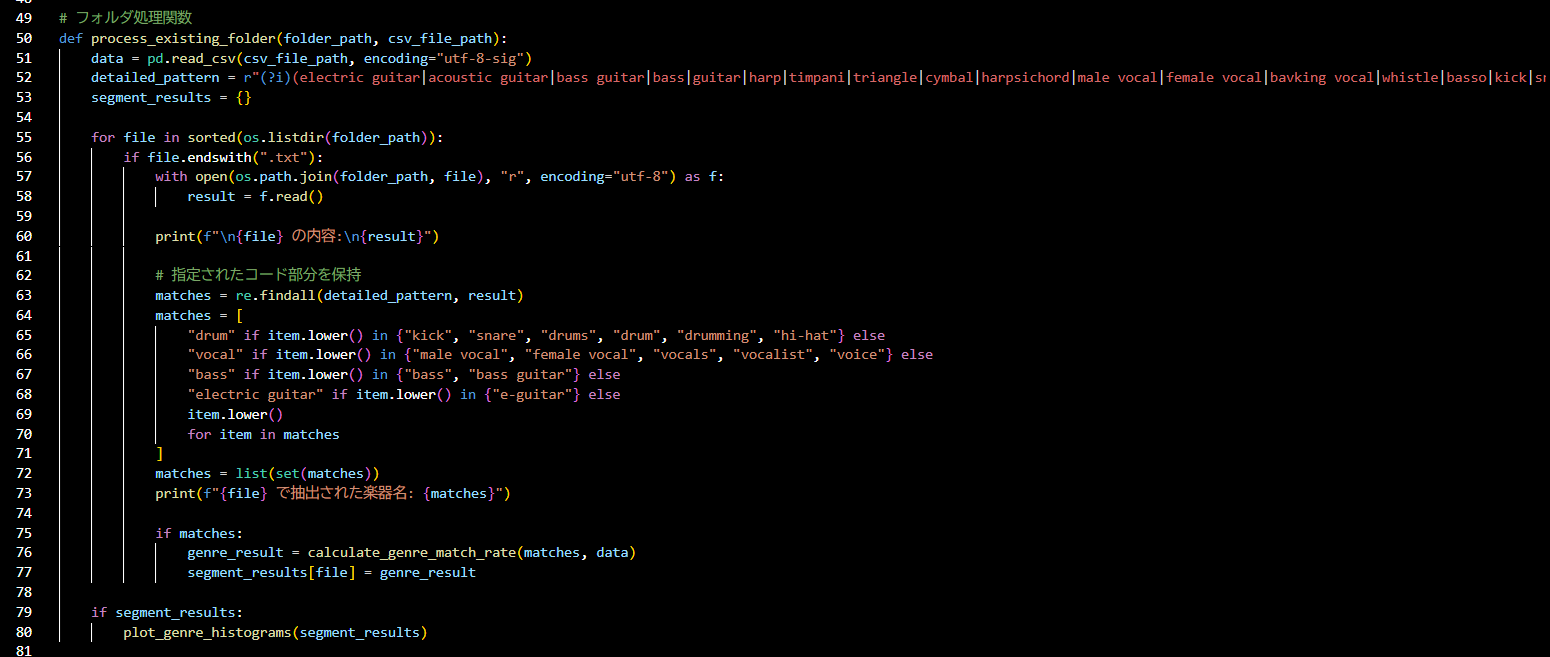
\includegraphics[width=\hsize]{fig/fig8-folder.png}
	  \caption{Process-existing-folder関数のソースコード}
	  \label{fig:text}
\end{figure}

引数は”folder-path”（処理対象のフォルダパス），”csv-file-path”（csvファイルのパス）である．

本システムでは，楽器名を正規表現パターンと定義して使用楽器を抽出している．
取得した各テキストファイルの内容を小文字に変換後，正規表現で楽器名を抽出する．
その際，一部の楽器名は一般的なカテゴリに変換する処理を追加した．

次に，データベースと一致する楽器がある場合，”calculate-genre-match-rate”関数を用いて音楽ジャンルの一致率を計算する．

計算結果は”segment-results”辞書に保存され、”plot-genre-histograms”関数を用いて音楽ジャンルごとの一致率をヒストグラムで表示する．
この際，セグメントの音楽ジャンル一致率の計算結果を引数に取る．

\subsection{upload-file関数}
本関数は，ユーザが音声ファイルをアップロードするための関数である．
関数のソースコードを\figref{fig:upload}に示す．

\begin{figure}[tb]
	  \centering
	  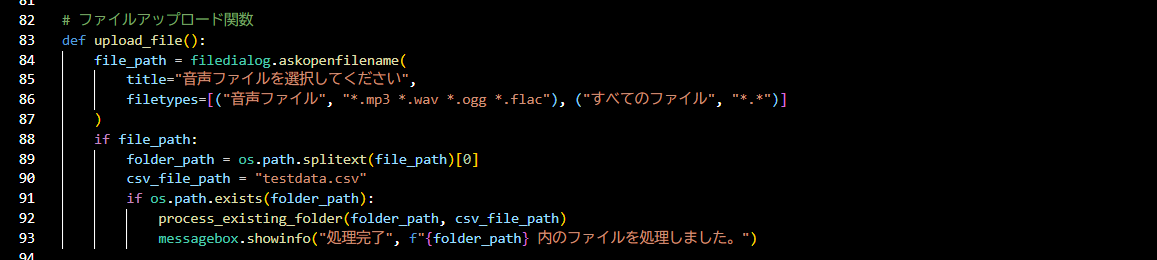
\includegraphics[width=\hsize]{fig/fig9-upload.png}
	  \caption{upload-file関数のソースコード}
	  \label{fig:text}
\end{figure}

本システムの入力はmp3であるため，選択可能なファイル形式は.mp3のみに指定している．
また、データベースは固定のパスとして設定している．

指定パスが存在し，ディレクトリであるかを確認後，指定フォルダ内のテキストファイルを処理する．
処理内容はprocess-existing-folder関数の内容である．

フォルダが存在しない場合，つまり解析したことのないファイルを解析する場合には以下の処理に分岐する．
Split-audio-to-named-dir関数を用いて音声ファイルを５秒ごとのセグメントに分割する．
分割されたセグメントを，webサイトを介して処理する．

\subsection{GUIの構築}
ソースコードを\figref{fig:HUI}に示す．

\begin{figure}[tb]
	  \centering
	  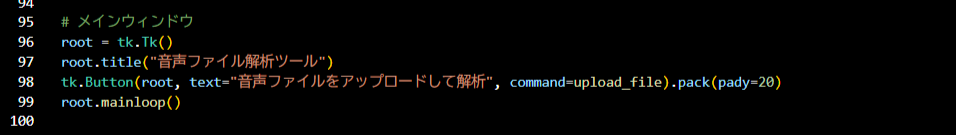
\includegraphics[width=\hsize]{fig/fig10-HUI.png}
	  \caption{GUIのソースコード}
	  \label{fig:text}
\end{figure}

GUIはtkinterを用いて作成する．

ウィンドウのタイトルバーに表示される文字列を「音声ファイル解析ツール」に設定する．
プログラムを実行すると，音声ファイルのアップロードボタンがウィンドウに表示される．

その他のGUIは各関数で処理内容を記述している．



\section{検証}
本章では，構築したシステムの検証手順とその結果を記述する．

\subsection{「Slow Motion Dream」での検証} 
入力する楽曲は，Steven M Bryantの「Slow Motion Dream」の一部を使用する．
この楽曲は，インターネット上で公開されているフリーミュージックである．
この音声ファイルは序盤はelectric guitar，vocalで構成され，途中でdrumが加わる楽器構成である．
音声ファイルの時間は約10秒である．

検証結果のヒストグラムを\figref{fig:example_jazz}，\figref{fig:example_rock}，\figref{fig:example_classic}に示す．

\begin{figure}[tb]
	  \centering
	  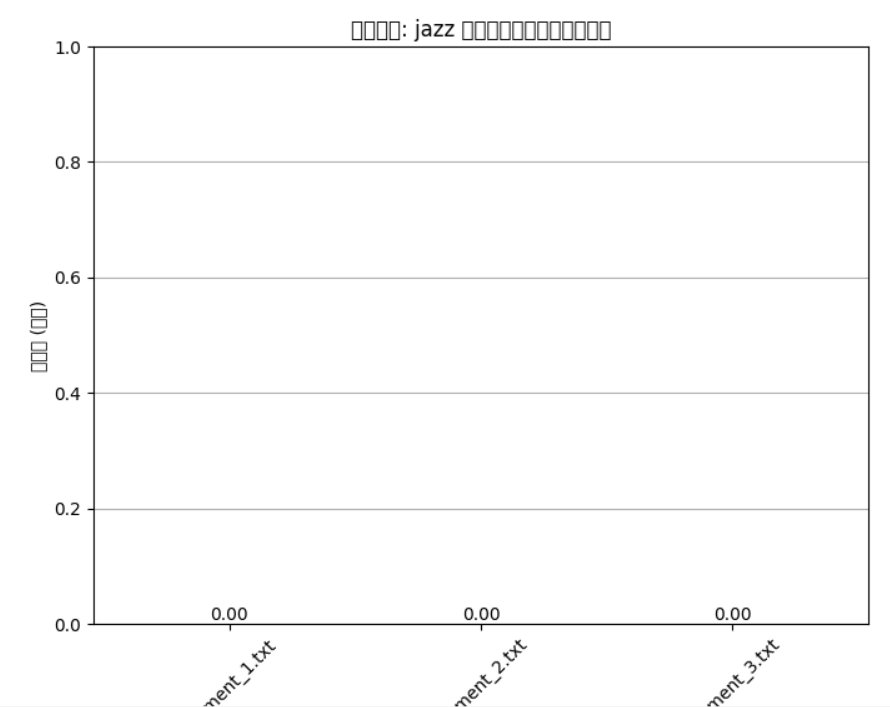
\includegraphics[width=\hsize]{fig/fig13-example_jazz.png}
	  \caption{Slow Motion Dreamのjazzヒストグラム}
	  \label{fig:text}
\end{figure}

\begin{figure}[tb]
	  \centering
	  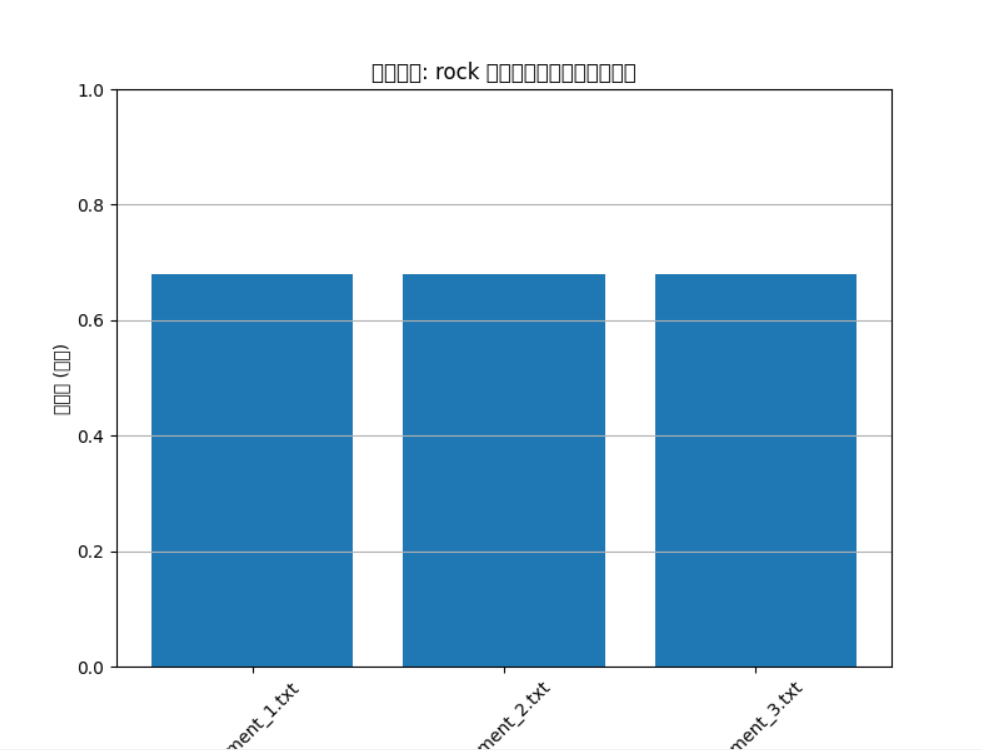
\includegraphics[width=\hsize]{fig/fig14-example_rock.png}
	  \caption{Slow Motion Dreamのrockヒストグラム}
	  \label{fig:text}
\end{figure}

\begin{figure}[tb]
	  \centering
	  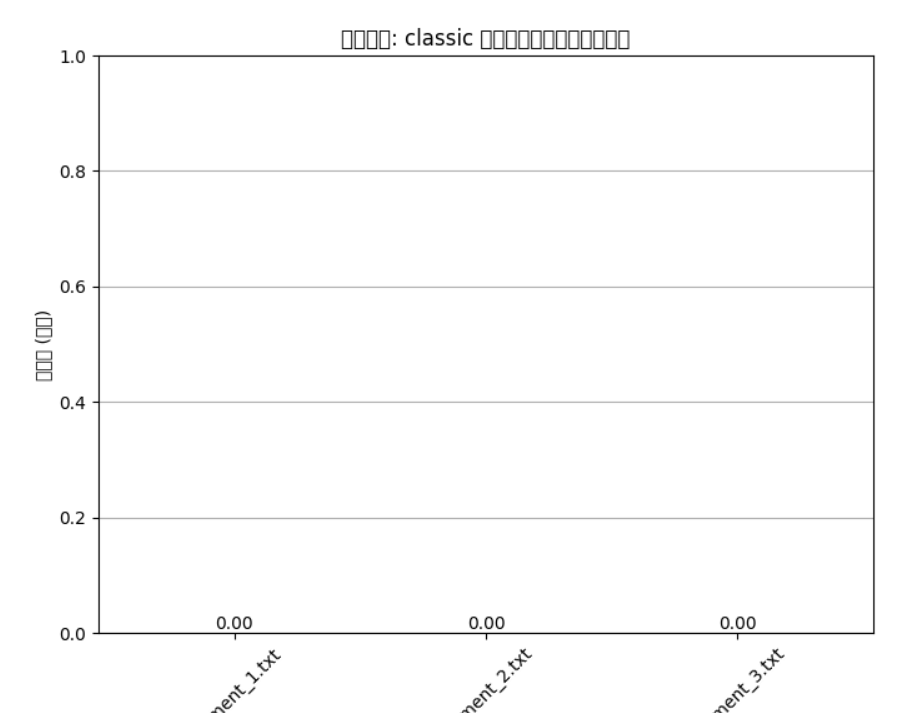
\includegraphics[width=\hsize]{fig/fig12-example_classic.png}
	  \caption{Slow Motion Dreamのclassicヒストグラム}
	  \label{fig:text}
\end{figure}

\figref{fig:segment1_txt}，\figref{fig:segment2_txt}，\figref{fig:segment3_txt}は，各セグメントで取得されたテキストファイルの内容である．

\begin{figure}[tb]
	  \centering
	  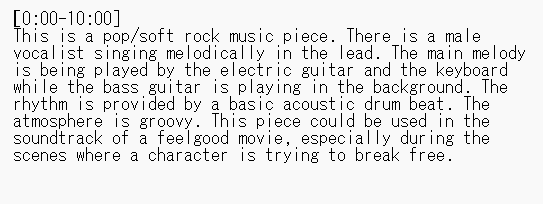
\includegraphics[width=\hsize]{fig/fig15-segment1_txt.png}
	  \caption{0秒から5秒で取得したテキスト}
	  \label{fig:text}
\end{figure}

\begin{figure}[tb]
	  \centering
	  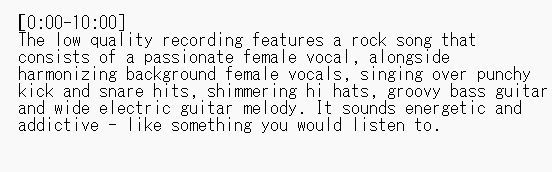
\includegraphics[width=\hsize]{fig/fig16-segment2_txt.png}
	  \caption{5秒から10秒で取得したテキスト}
	  \label{fig:text}
\end{figure}

\begin{figure}[tb]
	  \centering
	  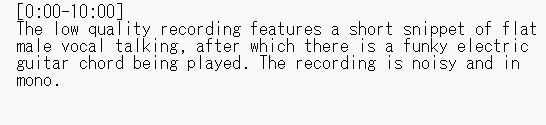
\includegraphics[width=\hsize]{fig/fig17-segment3_txt.png}
	  \caption{10秒からおわりまでで取得したテキスト}
	  \label{fig:text}
\end{figure}

また，このテキストから取得した楽器構成は次のとおりである．

・0秒から5秒：['vocal', 'electric guitar', 'bass guitar']

・5秒から10秒：['vocal', 'electric guitar', 'drum', 'bass guitar']

・10秒からおわり：['vocal', 'electric guitar']

これらの楽器構成はすべて聴取した際の楽器構成と一致しており，楽器構成や一致率の計算結果，ヒストグラムの結果は正しいといえる．

\subsection{「EMPIRE」での検証}
入力する楽曲はsnowmanの「EMPIRE」冒頭1分19秒を使用する．

この楽曲はモーツァルト作曲「交響曲第25番ト短調K.183」の第一楽章をサンプリングした楽曲であり，イントロと呼ばれる冒頭部分ではサンプリング元楽曲の冒頭部分である第一楽章の第一主題が流れ，その後ロック調のメロディで構成される．
また，間奏部分においてもサンプリング元楽曲が流れており，classicとjazzの要素が時間水位に伴い混在する楽曲となっている．
このように本楽曲は時間遷移に伴いジャンルが変化しているため，システムの検証に適していると考えた．

検証結果のヒストグラムを\figref{fig:EMPIRE_short_jazz}，\figref{fig:IMPIRE_short_rock}，\figref{fig:EMPIRE_short_classic}に示す．

\begin{figure}[tb]
	  \centering
	  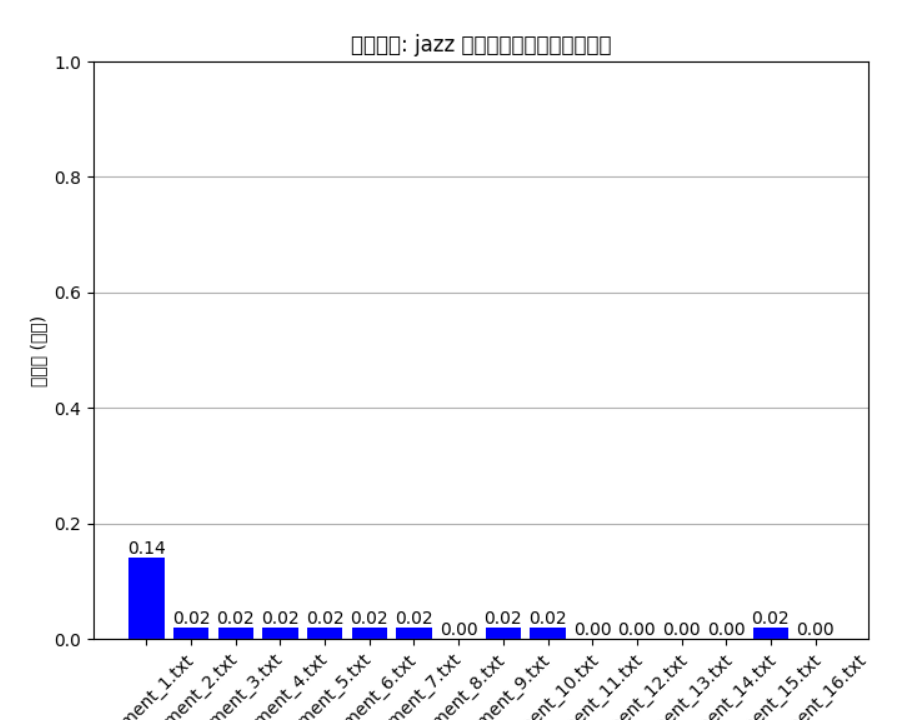
\includegraphics[width=\hsize]{fig/fig3-EMPIRE_short_jazz.png}
	  \caption{EMPIREのjazzヒストグラム}
	  \label{fig:text}
\end{figure}

\begin{figure}[tb]
	  \centering
	  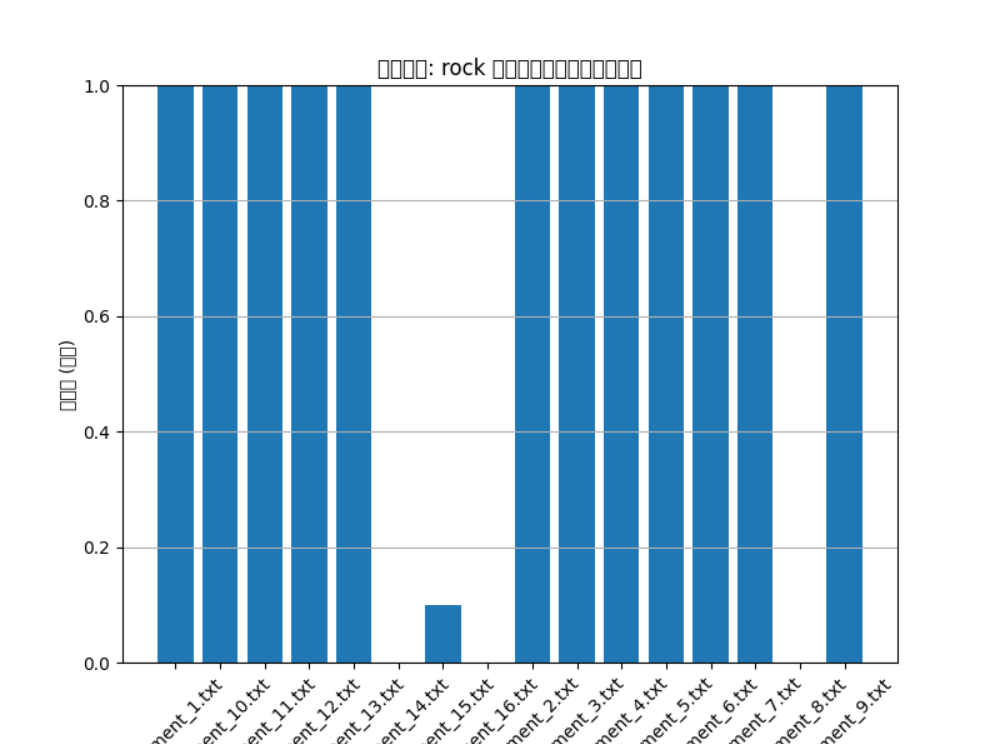
\includegraphics[width=\hsize]{fig/fig2-EMPIRE_short_rock.png}
	  \caption{EMPIREのrickヒストグラム}
	  \label{fig:text}
\end{figure}

\begin{figure}[tb]
	  \centering
	  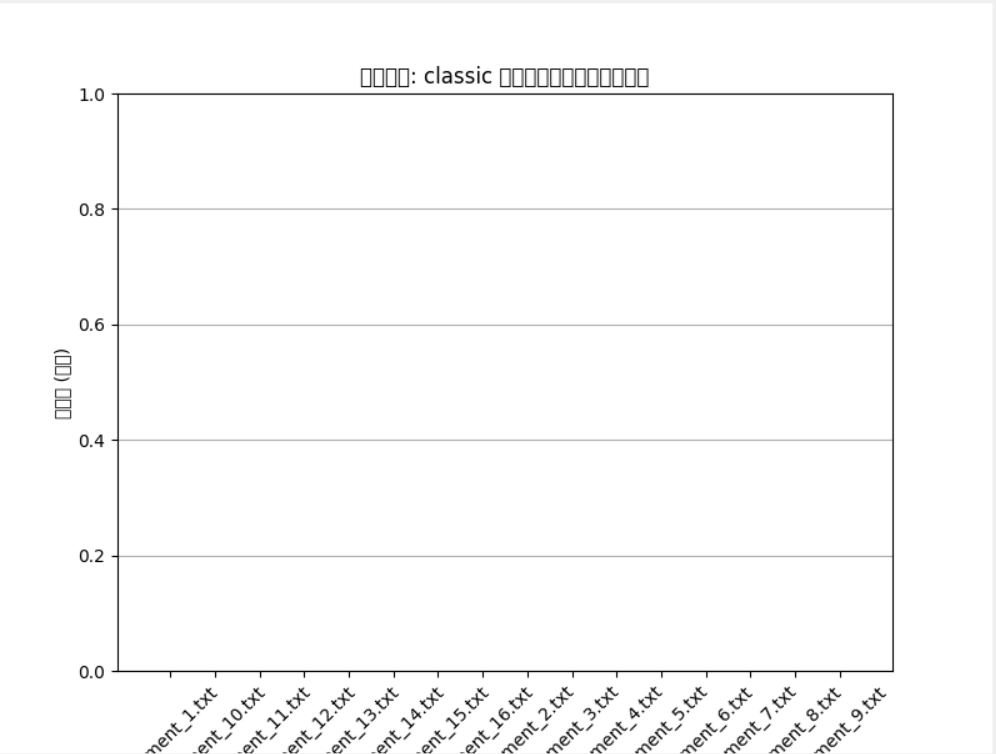
\includegraphics[width=\hsize]{fig/fig1-EMPIRE_short_classic.png}
	  \caption{EMPIREのclassicヒストグラム}
	  \label{fig:text}
\end{figure}

対象楽曲の冒頭5秒間の楽器構成はviolin，viola，cello，contrabass，oboe，faggot，corn，horn，vocal，drumである．
そのため，classicの一致度が高くなることが考えられた．

しかし，実装結果はclassicの一致度が0となっている．
データベースのClassic楽曲にはvocalが使用されている楽曲がないため，このような結果が出ていると考えられる．

また，冒頭5秒間のセグメントにて取得した楽器構成リストは，['vocal']のみである．
対象楽曲で試用されている楽器数が多いため，テキスト生成の際に正確に楽器を抽出できなかったものと考えられる．



\section{今後の課題}
本システムでは音色の抽出にLP-MusicCapsを使用したが，楽器数が多いと正確に使用楽器が抽出できないという問題点があった．
そのため，楽器数の少ない楽曲を対象楽曲とした際は正しい結果が得られたが，音数が多く複雑な楽曲を対象楽曲とした際に正しい実装結果が得られなかった．

今後の課題として，音色の抽出方法の見直しがあげられる．

また，今回は50曲×3の150曲のデータベースを使用した．
しかし，より正確かつ汎用性の高いシステムになるために，データベースの拡大が必要であると考える．



\section{おわりに}
本研究では，楽曲中の時間推移に伴う音楽ジャンルの変化を分析・可視化するシステムを提案し，検証を行った．
従来の1つの楽曲を1つの音楽ジャンルに分類する解析手法では捉えきれなかったジャンルの多様性に注目し，楽器構成の変化を時間軸に沿って解析することで，楽曲内でジャンルがどのように移り変わるかを可視化する新しいアプローチを示した．

検証の結果，楽器構成がシンプルな楽曲では有効な結果を得られたが，楽器構成が複雑な楽曲では音色抽出の精度に課題があることが明らかになった．
例えば、特定の楽器が正確に認識されないず，データベースとの一致率に影響を及ぼすケースが確認された．
また，今回使用したデータベースは150曲と規模が限られており，データの多様性においても改善の余地があると考える．

今後の課題として，音色抽出アルゴリズムの改良や，より大規模で多様性に富んだデータベースの構築が挙げられる．
これにより，複雑な楽曲への対応力を向上させるとともに，システムの汎用性と精度を高めることが可能となる．

本研究は，音楽ジャンル解析における新たな視点を提供し，音楽の多様性を捉える手法の一端を示した．
本システムが音楽理解の深化や楽しみ方の多様化に寄与することを期待する． 



\begin{acknowledgment}
    %本稿の執筆にあたり，参考文献に挙げた方々のWebサイト，スライド，各種資料を大いに参考にさせていただいた．
    書くならお好きに
\end{acknowledgment}

